
% \subsection*{subsection name}
%
% we choose $\q(\nuk \vert \eta)$ to be logit-normally distributed,
% and express the expectations in \eqref{stick_expectations} as Gaussian integrals.
% Define
% \begin{align*}
%   \tilde \nuk := \log\left(\frac{\nuk}{1 - \nuk}\right),
% \end{align*}
% which will be normally distributed under our choice of a
% logit-normal $\q(\nuk \vert \eta)$.
%
% Let $\lnumean_\k$ and $\lnusd_\k$ be entries of $\eta$ corresponding to
% the logit-normal parameters of $\nuk$.
%
%
% In order to optimize the variational objective \eqref{vb_optimization} we see
% from \eqref{stick_log_post} that we need to evaluate or approximate expectations
% of the form
% %
% \begin{align*}
% %
% \expect{\q(\nuk \vert \eta)}{\log \nuk}
% \textrm{,}\quad
% \expect{\q(\nuk \vert \eta)}{\log (1 - \nuk)}
% \textrm{,}\quad\textrm{and}\quad
% \expect{\q(\nuk \vert \eta)}{\log \pstick(\nuk)}.
% %
% \end{align*}
%
%
%
%
% First, define a version of $\nuk$ that is not constrained to $(0,1)$:
% %
% \begin{align}\eqlabel{lnuk_transform}
% %
% \lnuk :={} \log \left( \frac{\nuk}{1 - \nuk} \right)
% \quad\Leftrightarrow\quad
% \nuk :={} \frac{\exp(\lnuk)}{1 + \exp(\lnuk)}.
% %
% \end{align}
% %
It will be useful later to have at hand the transform between densities
expressed in the space of $\nu$ and $\lnu$, which is given by
%
\begin{align}\eqlabel{lnuk_derivatives}
%
\fracat{d \lnu_\k}{ d\nuk}{\nuk} ={}
%     \frac{1-\nuk}{\nuk}
%     \left(\frac{1}{1 - \nuk} + \frac{\nuk}{(1 - \nuk)^2} \right)
% \\={}& \frac{1}{\nuk} + \frac{1}{1 - \nuk}
% \\={}&
    \frac{1}{\nuk (1 - \nuk)} \mathand
%
\fracat{d \nuk}{ d\lnuk}{\lnuk} ={}
    \frac{\exp(\lnuk)}{(1 + \exp(\lnuk))^2}.
%
\end{align}
% %
% We wish to let $\lnu_\k$ be distributed normally under the variational
% distribution.  Let $\lnumean_\k$ and $\lnusd_\k$ be entries of the parameter
% vector $\eta$, and write
% %
% \begin{align}\eqlabel{lnuk_vb_approximation}
% %
% \q(\lnu_\k \vert \eta) ={}& \normdist{\lnu_\k \vert \lnumean_\k, \lnusd_\k}
% \Rightarrow \\
% \q(\nuk \vert \eta) ={}&
%     \normdist{\log \left( \frac{\nuk}{1 - \nuk} \right)
%         \vert \lnumean_\k, \lnusd_\k}
%     \left|\fracat{d \lnu_\k}{ d\nuk}{\nuk}\right|
% \nonumber\\={}&
% \normdist{\log \left( \frac{\nuk}{1 - \nuk} \right)
%         \vert \lnumean_\k, \lnusd_\k}
%     \left|\frac{1}{\nuk (1 - \nuk)}\right|.
% \nonumber
% %
% \end{align}
% %
% Given this, we can approximate expectations of smooth functions
% $f(\nuk)$ using GH quadrature with $\ngh$ knots,
% located at $\xi_g$, weighted by $\omega_g$:
% %
% \begin{align}\eqlabel{gh_integral}
% %
% \expect{\q(\nuk \vert \eta)}{f(\nuk)} ={}&
% \expect{\q(\lnu_\k \vert \eta)}
%        {f\left(\frac{\exp(\lnu_\k)}{1 + \exp(\lnu_\k)}\right)}
% \nonumber\\\approx{}&
%     \sum_{g=1}^{\ngh} \omega_g f\left(\lnusd_\k \xi_{g} + \lnumean_\k\right)
%  \nonumber\\=:{}&
% \expecthat{\q(\nuk \vert \eta)}{f(\nuk)}.
% %
% \end{align}
% %
% Conveniently, $\expecthat{\q(\nuk \vert \eta)}{f(\nuk)}$ is a differentiable
% function of $\lnumean_\k$ and $\lnusd_\k$, and so also of $\eta$.  (This
% technique is similar to the ``reparameterization trick,'' only using
% GH points rather than standard normal draws.)

\hrulefill

In the regression example (\exref{mice_bnp_process}), $\zeta$ includes
the additive shifts, $\zeta := (\beta, \z, \nu, \b)$.

The variational approximation for the topic model
(\exref{structure_bnp_process}) is similarly mean-field: the distribution on
stick-breaking proportions $\nu$ factorizes over both individuals $\n$ and
components $\k$, while the assignments $\z$ factorize over individuals $\n$,
loci $\l$, and chromosomes $\i$. For the regression model
(\exref{mice_bnp_process}), all terms in the variational approximation
fully-factorize except for the cluster assignments $\z$ and additive shifts
$\b$. While we assume $(\z, \b)$ to be independent from all other latent
variables under $\q$, we will allow conditional dependence between $\z$ and $\b$
(\appref{app_mice}).




\hrulefill


% This is necessary here becuase it is a condition under which we have
% differentiability.  Alternatively, we could define it later when
% stating our differentiability theorem...
The KL divergence of \eqref{kl_def} contains a term of the form $\expect{\q(\nuk
\vert \eta)}{\log \pstick(\nuk)}$.  Since we will be considering generic
densities $\pstick(\nuk)$, we will need to compute this integral numerically.
To facilitate numerical integration, we model the sticks using a logit-normal
distribution as follows.  Define
%
\begin{align*}
%
\lnuk := \log\left(\frac{\nuk}{1 - \nuk}\right),
%
\end{align*}
%
and choose $\q(\lnu_\k \vert \eta)$ to be normally distributed.  This then
induces a logit-normal distribution on our original variable of interest,
$\nuk$.  See \secref{stick_expectations} below for more details.




\hrulefill




%%%%%%%%%%%%%%%%%%%%%%%%%%%%%%%%%%%%%%%%%%%%%%%%%%%%%%%%%%%%%%%%%%%%%%%%%%%%

We conclude this section with a brief remark about computing the expectation
$\crosshessian$ in our BNP sensitivity analysis.
We are interested in sensitivity to the stick-breaking distribution,
so only the prior terms on stick-breaking proportions
$\nu = (\nu_1, ..., \nu_{\kmax - 1})$ depends on $t$.
Because the elements of $\nu$ fully factorize
under both the prior and the variational distributions,
$\crosshessian$ decomposes as
\begin{align}
  \crosshessian &=
  \sum_{\k=1}^{\kmax - 1}
          \expect{\q(\nuk \vert \eta)}
                 {
                 \lqgrad{\nuk \vert \etaopt}
                 \fracat{\log \pstick(\nuk \vert \t)}{\partial \t}{\t = 0}
                 } \notag\\
  &= \sum_{\k=1}^{\kmax - 1}
         \evalat{\nabla_\eta \expect{\q(\nuk \vert \eta)}
                {
                \fracat{\log \pstick(\nuk \vert \t)}{\partial \t}{\t = 0}
                }}{\eta = \etaopt(0)},
\eqlabel{sens_mixed_partial}
\end{align}
where we assumed that $\q(\theta \vert \eta)$ is normalized, so
$\lqgradbar{\theta \vert \etaopt} = \lqgrad{\theta \vert \etaopt}$,
and that the assumptions of \thmref{etat_deriv} hold, so we
can freely exchange derivatives with expectations.

We approximate the expectation using GH quadrature (\eqref{gh_integral}), with
$f(\nu_k) = \fracat{\log \pstick(\nuk \vert \t)}{\partial \t}{\t = 0}$. In all
the functional forms for $\t \mapsto \pstick(\nuk \vert \t)$ considered below,
$f(\nu_k)$ can be provided in either closed-form or computed with automatic
differentiation. The resulting GH approximation is a deterministic function of
$\eta$, and thus the gradient in \eqref{sens_mixed_partial} can be computed with
another application of automatic differentiation. Note that $\crosshessian$ is
sparse in \eqref{sens_mixed_partial}: it is zero for all entries of $\eta$ other
than those that parameterize the sticks.


\hrulefill

\subsection{Function-valued prior perturbations}
\seclabel{functional_perturbations}
In \corref{gem_approximation_ok} of \secref{local_sensitivity}, we showed that
we can form a Taylor series approximation to the dependence of a variational
optimum on the parameter $\alpha$ in a Beta prior. However, there is typically
no {\em a priori} reason to believe that the stick breaking prior lies within
the parametric Beta family.  In this section, we follow
\citet{gustafson:1996:local} and define a class of ways to perturb to the
functional form of the prior, corresponding to the $\lp{p}$ classes of
integrable functions (which we will define and discuss below).

For any particular perturbation, \thmref{etat_deriv} can be applied directly by
verifying \assuref{q_stick_regular}.  However, we will argue that it is
typically more useful to examine the form of the derivative to find influential
perturbations, for which one wants a stronger result than can be provided
by \thmref{etat_deriv} alone---we will require that the derivatives give
{\em uniformly good linear approximations} within bounded sets.
We address this question in \secref{differentiability}.

Let us remain with the general problem of inference on a parameter $\theta$. Fix
a base prior density, $\pbase(\theta)$, at which we have computed a VB
approximation.  Suppose we wish to ask what the variational optimum would have
been had we used some alternative prior density, $\palt(\theta)$.  Let us write
$\etaopt(\pbase)$ and $\etaopt(\palt)$ for these two approximations,
respectively.  To approximately answer this question using the local sensitivity
approach of \secref{local_sensitivity}, we must somehow define a continuous path
from $\pbase(\theta)$ to $\palt(\theta)$ parameterized, say, by $\t \in [0, 1]$.

There are many ways to do so.  For example, one might form the mixture
distribution:
%
\begin{align*}
%
\p_{lin}(\theta \vert \t) =
    (1- \t) \pbase(\theta) + \t \palt(\theta).
%
\end{align*}
%
Then $\p_{lin}(\theta \vert \t=0) = \pbase(\theta)$, $\p_{lin}(\theta \vert \t=1) =
\palt(\theta)$, and $\p_{lin}(\theta \vert \t)$ interpolates smoothly between the
two.  We could then attempt to apply \thmref{etat_deriv} using $\pstick(\nu \vert
\t)$ to compute $d\etaopt(\t) / d\t$, and approximate
%
\begin{align*}
%
\etaopt(\palt) \approx \etaopt(\pbase) + \fracat{d \etaopt(\t)}{d\t}{\t=1}(1 - 0).
%
\end{align*}
%
However, we might alternatively have defined the mixture in the log densities:
%
\begin{align*}
%
\log \p_{mult}(\theta \vert \t) =
    (1- \t) \log\pbase(\theta) + \t \log\palt(\theta) -
    \const. \\ \constdesc{\theta}
%
\end{align*}
%
Again, $\p_{mult}(\theta \vert \t=0) = \pbase(\theta)$, $\p_{mult}(\theta \vert
\t=1) = \palt(\theta)$, and $\p_{mult}(\theta \vert \t)$ interpolates smoothly
between the two.

Indeed, one may define a family of prior perturbations by adding the densities
after transforming pointwise by any invertible transformation, and then
transforming back into the original space.  We will consider (a generalization
of) the family of ``nonlinear'' functional perturbations given by
\citep{gustafson:1996:local}, of which our examples $\p_{lin}$ and $\p_{mult}$
are the two extremes, corresponding to $p=1$ and $p=\infty$, respectively.

Below, we will take $\lambda$ to denote the Lebesgue measure on the Borel sets
of $\thetadom \subseteq \mathbb{R}^{\thetadim}$.  We will be interested in
densities with respect to $\lambda$, expressed as Radon-Nikodym derivatives,
though it will be convenient to use the same notation for a density and for the
measure induced by the density.  Specifically, for a $\lambda$-measurable set
$S$, and a Radon-Nikodym derivative $f$ defined with respect to $\lambda$, we
will write $f(S) = \int_{\theta \in S} f(\theta) \lambda(d\theta)$.  Similarly,
for two densities $f$ and $g$, we will write $f \ll g$ to mean that $g(S) = 0
\Rightarrow f(S) = 0$ for all $\lambda$-measurable sets $S$.

%%%%%%%%%%%%%%%%%%%%%%%%%%%%%%%%%%%%%%%%%%%%%%%%%%%%%%%%%%%%%%%%%%%%%%%%%
%%%%%%%%%%%%%%%%%%%%%%%%%%%%%%%%%%%%%%%%%%%%%%%%%%%%%%%%%%%%%%%%%%%%%%%%%
\begin{defn}\deflabel{prior_nl_pert}
%
Fix $\pbase(\theta)$, a density with respect to $\lambda$, and fix $1 \le p \le
\infty$.  Assume that $\pbase(\theta) > 0$ on $\thetadom$. For any
$\phi(\theta)$ for which the expressions are well-defined, let
%
\begin{align*}
%
\rho(\theta \vert \phi) :={}& \begin{cases}
%
\pbase(\theta)^{1/p} + \frac{1}{p}\phi(\theta)
    & \textrm{when }p \in [1, \infty) \\
\pbase(\theta)\exp(\phi(\theta))
    & \textrm{when }p = \infty
%
\end{cases}\\
%
\tilde{\p}(\theta \vert \phi) :={}&
    \mathrm{sign}(\rho(\theta \vert \phi)) \abs{\rho(\theta \vert \phi)}^p\\
\p(\theta \vert \phi) :={}&
    \frac{\tilde{\p}(\theta \vert \phi)}
         {\int \tilde{\p}(\theta' \vert \phi) d\theta'}.
%
\end{align*}
%
\end{defn}
%
%%%%%%%%%%%%%%%%%%%%%%%%%%%%%%%%%%%%%%%%%%%%%%%%%%%%%%%%%%%%%%%%%%%%%%%%%

We have specified \defref{prior_nl_pert} in terms of the general function
$\phi(\theta)$ rather than an alternative $\palt(\theta)$.  The reason is so
that the perturbed prior $\p(\theta \vert \phi)$ is well-defined for $\phi$ that
may not be probabilities densities.  As we will soon show, this allows us to
embed $\phi$ in a vector space, in which $\p(\theta \vert \phi)$ is well-defined
in an open neighborhood of the zero function.

Nothing has been lost, however, since one can extrapolate to any alternative
density $\palt(\theta)$ by taking $\phi$ as given in the following definition.

%%%%%%%%%%%%%%%%%%%%%%%%%%%%%%%%%%%%%%%%%%%%%%%%%%%%%%%%%%%%%%%%%%%%%%%%%%%
%%%%%%%%%%%%%%%%%%%%%%%%%%%%%%%%%%%%%%%%%%%%%%%%%%%%%%%%%%%%%%%%%%%%%%%%%%%

\begin{defn}\deflabel{prior_pert_class}
%
Fix the quantities in \defref{prior_nl_pert}.  Fix a density $\palt(\theta)$
with respect to $\lambda$, with $\palt \ll \pbase$. For a given $\beta > 0$, let
%
\begin{align}
%
\phi(\theta | \beta, \palt) :={}
\begin{cases}
\beta \palt(\theta)^{1/p} - p \pbase(\theta)^{1/p}
    & \textrm{when }p \in [1, \infty) \\
\log \palt(\theta) - \log \pbase(\theta)
    & \textrm{when }p = \infty.
\end{cases} \eqlabel{phi_for_palt}
%
\end{align}
%
Similarly, define
%
\begin{align*}
%
% \pertset := \bigg\{&
%     \phi:     \phi \in \lp{\lambda, p} \textrm{ and }
%     \phi(\theta) = \beta \palt(\theta)^{1/p} - p \pbase(\theta)^{1/p}\\&
%     \textrm{ for some }\beta > 0\textrm{ and some density }\palt
% \bigg\}.
\pertset := \bigg\{&
    \phi:  \phi(\theta | \beta, \palt) %\\&
    \textrm{ for some }\beta > 0\textrm{ and some density }\palt
    \textrm{ with } \palt \ll \pbase
\bigg\}.
%
\end{align*}
%
% For notational convenience, when $p = \infty$, we simply take $\pertset =
% \lp{\lambda, \infty}$.\footnote{
% Observe that
% %
% %\begin{align*}
% %
% $\phi(\theta) = \beta \log \palt(\theta) - \log \pbase(\theta) \Rightarrow
% \palt(\theta) = \exp(\phi(\theta) / \beta) \pbase(\theta)^{1/\beta}.$
% %
% %\end{align*}
% %
% Since $\int \pbase(\theta)^{1/\beta} \lambda(d\theta)$ may be $\infty$, in
% general, there exist $\phi(\theta)$ which are of the form \eqref{phi_for_palt}
% when $p=\infty$.  It turns out that a restricted $\pertset$ will not be a useful
% concept when $p=\infty$, however.}
%
\end{defn}
%%%%%%%%%%%%%%%%%%%%%%%%%%%%%%%%%%%%%%%%%%%%%%%%%%%%%%%%%%%%%%%%%%%%%%%%%%%

The fact that we are free to choose $\beta$ follows from the fact that we
normalize after perturbing.  Note that multiplicative changes ($p=\infty$)
cannot produce alternatives $\palt(\theta)$ that are not mutually absolutely
continuous with $\pbase(\theta)$.


\begin{ex}
%
Take $\pbase(\theta) = \betadist{\theta \vert 1, \alpha_0}$ and
$\palt(\theta) = \betadist{\theta \vert 1, \alpha_1}$.  Then
$\thetadom=[0,1]$ and $\lambda$ is the Lebesgue measure on $[0,1]$, so
%
\begin{align*}
%
\pbase(\theta) ={}&
    \frac{\Gamma(\alpha_0)}{\Gamma(1 + \alpha_0)} (1 - \theta)^{\alpha_0 - 1}.
%
\end{align*}
%
Then, for $p = 1$,

\begin{align*}
%
\phi(\theta \vert \beta, \palt) ={}&
    \frac{\Gamma(\alpha_1)\beta}{\Gamma(1 + \alpha_1)} (1 - \theta)^{\alpha_1 - 1} -
    \frac{\Gamma(\alpha_0)}{\Gamma(1 + \alpha_0)}
        (1 - \theta)^{\alpha_0 - 1}.
%
\end{align*}
%
Note that, when $\t = 1$, the normalizing constant and $\beta$ cancel in the
normalization of $\p(\theta \vert \t \phi)$:
%
\begin{align*}
%
\p(\theta \vert \phi(\theta \vert \beta, \palt)) =
\frac{\frac{\Gamma(\alpha_1)\beta}{\Gamma(1 + \alpha_1)} (1 - \theta)^{\alpha_1 - 1}}
     {\frac{\Gamma(\alpha_1)\beta}{\Gamma(1 + \alpha_1)}
       \int_0^1 (1 - \theta')^{\alpha_1 - 1} \lambda(d\theta')}
=
\frac{(1 - \theta)^{\alpha_1 - 1}}
     {\int_0^1 (1 - \theta')^{\alpha_1 - 1} \lambda(d\theta')}.
%
\end{align*}
%
For this reason, we are free to choose $\beta > 0$ in \defref{prior_pert_class}
and still extrapolate to the same $\palt$ when $\t = 1$.

When $p = \infty$,
%
\begin{align*}
%
\phi(\theta \vert \beta, \palt) ={}&
    \log \left(
        \frac{\Gamma(\alpha_1) }{\Gamma(1 + \alpha_1)}
    \right)  + (\alpha_1 - 1) \log (1 - \theta) - \\
{}&
    \log \left(
        \frac{\Gamma(\alpha_0)}{\Gamma(1 + \alpha_0)}
    \right) + (\alpha_0 - 1) \log (1 - \theta) \\
={}&
\log \left(
    \frac{\Gamma(\alpha_1) }{\Gamma(1 + \alpha_1)}
\right) -
\log \left(
    \frac{\Gamma(\alpha_0)}{\Gamma(1 + \alpha_0)}
\right) + (\alpha_1 - \alpha_0) \log(1 - \theta).
%
\end{align*}
%
For $p = \infty$, the normalizing constant cancels for all $\t$:
%
\begin{align*}
%
\p(\theta \vert \t \phi(\theta \vert \beta, \palt)) ={}&
\frac{    \frac{\Gamma(\alpha_1) \Gamma(1 + \alpha_0) }
               {\Gamma(1 + \alpha_1) \Gamma(\alpha_0)}
        (1-\theta)^{\alpha_0 (1 - \t) + \alpha_1 \t}
    }
     {
     \frac{\Gamma(\alpha_1) \Gamma(1 + \alpha_0) }
          {\Gamma(1 + \alpha_1) \Gamma(\alpha_0)}
             \int_0^1 (1-\theta')^{\alpha_0 (1 - \t) +
                                   \alpha_1 \t} \lambda(d\theta')
     }
\\={}&
\frac{(1-\theta)^{\alpha_0 (1 - \t) + \alpha_1 \t}}
     {\int_0^1 (1-\theta')^{\alpha_0 (1 - \t) + \alpha_1 \t} \lambda(d\theta')}.
%
\end{align*}
%
\end{ex}


\begin{ex}
%
Take $\thetadom = [0,1]$.  The pair $\pbase(\theta)  = \frac{1}{2}\ind{\theta < 1/2}$
and $\palt(\theta) = \frac{1}{2} \ind{\theta > 1/2}$ are disallowed
by \defref{prior_pert_class} because we do not have $\palt \ll \pbase$.
%
\end{ex}


\begin{ex}
%
Equivalent densities can be given in different spaces via invertible
transformations.  Since the base measure of \defref{prior_nl_pert}
is fixed to the Lebesgue measure, the corresponding $\phi$ may be different.

Consider the logistic transform given by \eqref{lnuk_transform}. Let
$\p_{\nuk}(\nuk)$ be a density with respect to the Lebesgue measure on $[0,1]$,
and let $\p_{\lnuk}(\lnuk)$ be the corresponding density with respect to the
Lebesgue measure on $(-\infty, \infty)$.  By the ordinary rule for
transformation of densities and \eqref{lnuk_derivatives},
%
\begin{align*}
%
\p_{\lnuk}(\lnuk) = \p_{\nuk}(\nuk(\lnuk)) \frac{\exp(\lnuk)}{(1 +
\exp(\lnuk))^2}.
%
\end{align*}
%
\end{ex}

The classes of perturbations given in \defref{prior_nl_pert} have a natural
correspondence with the $\lp{\lambda, p}$ spaces of functions, which we now
define.

%%%%%%%%%%%%%%%%%%%%%%%%%%%%%%%%%%%%%%%%%%%%%%%%%%%%%%%%%%%%%%%%%%%%%%%%%%%
%%%%%%%%%%%%%%%%%%%%%%%%%%%%%%%%%%%%%%%%%%%%%%%%%%%%%%%%%%%%%%%%%%%%%%%%%%%

\begin{defn}\deflabel{lp_spaces}
\citep[Sections 5.1-5.2]{dudley:2018:real}
%
For a measure $\mu$ and $p \in [1, \infty]$, let $\lp{\mu,p}$ define the
space of equivalence classes of real-valued $\mu$-measurable functions,
where two functions are equivalent if they disagree only on a set of
$\mu$-measure zero.

Let $\esssup_\theta^\mu$ denote the essential supremum over $\theta$ with
respect to the measure $\mu$. The norm on $\lp{\mu,p}$ is given by
%
\begin{align*}
%
\norm{\phi}_{\mu,p} :={}&
\begin{cases}
    \left(\int \abs{\phi(\theta)}^p \mu(d\theta)\right)^{1/p}
    & \textrm{when }p \in [1, \infty)\\
    \esssup_{\theta} \abs{\phi(\theta)}
    & \textrm{when }p = \infty
\end{cases}\\
%
\phi \in \lp{\lambda,p} \Leftrightarrow{}& \norm{\phi}_{\lambda,p} < \infty.
%
\end{align*}
%
When $\lambda$ is the  Lebesgue measure, we may simply write $\lp{\lambda,p} =
\lp{p}$ and $\norm{\cdot}_{p} = \norm{\cdot}_{\lambda,p}$.
%
Let $\ball_{\mu,p}(\epsilon) := \{\phi: \phi \in \lp{\mu, p},
\norm{\phi}_p < \epsilon \}$ denote the $\epsilon$-ball in $\lp{\mu, p}$.
%
\end{defn}

By \citep[Theorem 5.2.1]{dudley:2018:real}, $\lp{\mu,p}$ is a Banach
space (i.e., a complete, normed vector space).


%%%%%%%%%%%%%%%%%%%%%%%%%%%%%%%%%%%%%%%%%%%%%%%%%%%%%%%%%%%%%%%%%%%%%%%%%%%






% We argue that pointwise negative priors are no substantive problem, as long as
% normalizing integral is neither zero nor infinity, and as long as we do not
% extrapolate to negative alternatives $\palt(\theta)$.  (Indeed, embedding
% statistical problems in non-statisical vectors spaces is a venerable technique
% when applying functional analysis to statistics, see, e.g., \citet[Chapter
% 6]{serfling:2009:approximation}.)  In order to permit negative $\phi$, we thus
% state the following generalization of \citep[Result 2]{gustafson:1996:local}.
%
% %%%%%%%%%%%%%%%%%%%%%%%%%%%%%%%%%%%%%%%%%%%%%%%%%%%%%%%%%%%%%%%%%%%%%%%%%
% %%%%%%%%%%%%%%%%%%%%%%%%%%%%%%%%%%%%%%%%%%%%%%%%%%%%%%%%%%%%%%%%%%%%%%%%%
% \begin{lem}\lemlabel{pert_well_defined}
% %
% Fix a $1 \le p < \infty$ and $\pbase(\theta)$ as in \defref{prior_nl_pert}.
% For any $\phi \in \lp{\lambda,p}$ and $\norm{\phi}_{\lambda,p} < p$, then
% %
% \begin{align*}
% %
% 0 < \int \tilde{\p}(\theta \vert \phi) \lambda(d\theta) < \infty,
% %
% \end{align*}
% %
% so that $\int p(\theta \vert \phi) \lambda(d\theta) = 1$.
%
% Furthermore, for any $1 \le p \le \infty$, when $\phi \in \pertset$ and $0 \le
% \t \le 1$, then
% %
% \begin{align*}
% %
% \ptil(\theta \vert \t \phi) \ge{}& 0 \mathand\\
% 0 < \int \ptil(\theta \vert \t \phi) \lambda(d\theta) < \infty.
% %
% \end{align*}
% %
% (For a proof see \appref{proofs} \proofref{pert_well_defined}.)
% %
% \end{lem}
%
% %%%%%%%%%%%%%%%%%%%%%%%%%%%%%%%%%%%%%%%%%%%%%%%%%%%%%%%%%%%%%%%%%%%%%%%%%


%
% %%%%%%%%%%%%%%%%%%%%%%%%%%%%%%%%%%%%%%%%%%%%%%%%%%%%%%%%%%%%%%%%%%%%%%%%%
% %%%%%%%%%%%%%%%%%%%%%%%%%%%%%%%%%%%%%%%%%%%%%%%%%%%%%%%%%%%%%%%%%%%%%%%%%
% \begin{lem}\lemlabel{pert_well_defined}
% %
% Fix the quantities given in \defref{prior_nl_pert}, and let $0 \le \t \le 1$.
%
% First, consider $1 \le p < \infty$.  If $\phi \in \pertset$, then
% $\norm{\phi}_{\lambda,p} < \infty$, $\p(\theta \vert \t \phi) \ge 0$, and
% $\essinf_{\theta} \frac{\phi(\theta)}{\pbase(\theta)^{1/p}} \ge 0$. Furthermore,
% if $\phi \in \ball_{\lambda,p}(p)$ or if $\phi \in \pertset$, then $0 < \int
% \ptil(\theta \vert \phi) \lambda(d\theta) <{} \infty$.
%
% % However,
% % there may be $\phi$ with arbitrarily small $\norm{\phi}_{\lambda,p}$
% % and $\essinf_\theta \p(\theta \vert \phi) < 0$.
%
% For $p = \infty$, $\norm{\phi}_{\lambda,p} < \infty$ implies that $\p(\theta
% \vert \phi) \ge 0$ and $0 < \int \ptil(\theta \vert \phi) \lambda(d\theta) <{}
% \infty$.
%
% % However, there may be $\phi \in \pertset$ with $\norminf{\phi} =
% % \infty$.
%
% (For a proof see \appref{proofs} \proofref{pert_well_defined}.)
% %
% \end{lem}

%%%%%%%%%%%%%%%%%%%%%%%%%%%%%%%%%%%%%%%%%%%%%%%%%%%%%%%%%%%%%%%%%%%%%%%%%


\begin{lem}\lemlabel{pert_well_defined}
%
Fix the quantities given in \defref{prior_nl_pert}.  We have the following
relations between $\pertset$, $\lp{p}$, and the space of valid
prior densitites:
%
\begin{enumerate}
%
    \item If $\phi \in \pertset$, then $\p(\theta \vert \t \phi)$ is a valid
    density (non-negative and normalizable) for all $0 \le \t \le 1$.
%
    \item If $p \in [1, \infty)$, then $\pertset \subset
        \ball_{p}(p)$.
%
    \item If $p = \infty$, $\lp{\infty} \subset \pertset[\infty]$.
%
    % \item If $1 \le p < \infty$ and $\phi \in \pertset$, then
    % $\essinf_{\theta} \frac{\phi(\theta)}{\pbase(\theta)^{1/p}} \ge 0$.
%
\end{enumerate}
%
\end{lem}

%%%%%%%%%%%%%%%%%%%%%%%%%%%%%%%%%%%%%%%%%%%%%%%%%%%%%%%%%%%%%%%%%%%%%%%%%
% \/  \/  \/  \/  \/  \/  \/  \/  \/  \/  \/  \/  \/  \/  \/  \/  \/  \/
\begin{ex}\exlabel{beta_inf_norm}
%
It is possible for $\phi \in \pertset[\infty]$ to have $\norminf{\phi} =
\infty$, and so $\phi \notin \lp{\lambda,\infty}$.  Take $\lambda$ to be the
Lebesgue measure on $[0,1]$, let $\pbase(\theta) = \betadist{\theta \vert 1,
\alpha_0}$ and $\palt(\theta) = \betadist{\theta \vert 1, \alpha_1}$ for
$\alpha_0 \ne \alpha_1$.  Then $\phi(\theta) = (\alpha_1 - \alpha_0) \log(1 -
\theta) \log(1 - \theta)$
%
and
%
\begin{align*}
%
\norminf{\phi} =
    \abs{\alpha_1 - \alpha_0} \sup_{\theta \in [0,1]} \abs{\log(1 - \theta)} =
    \infty.
%
\end{align*}
%
\end{ex}
% /\    /\    /\    /\    /\    /\    /\    /\    /\    /\    /\    /\    /\
%%%%%%%%%%%%%%%%%%%%%%%%%%%%%%%%%%%%%%%%%%%%%%%%%%%%%%%%%%%%%%%%%%%%%%%%%%%%

%%%%%%%%%%%%%%%%%%%%%%%%%%%%%%%%%%%%%%%%%%%%%%%%%%%%%%%%%%%%%%%%%%%%%%%%%
% \/  \/  \/  \/  \/  \/  \/  \/  \/  \/  \/  \/  \/  \/  \/  \/  \/  \/
\begin{ex}\exlabel{lp_negative}
%
Suppose $\pbase$ induces a continuous measure, i.e., there exists a sequence
$\epsilon_n \rightarrow 0$ with $\epsilon_n > 0$ and a sequence of corresponding
sets such that $\pbase(S_n) = \epsilon_n$.  Then, for $1 \le p < \infty$, it is
possible for $\phi \in \ball_{\lambda,p}(\epsilon)$ for arbitrarily small
$\epsilon$ and yet have $\essinf_{\theta} \p(\theta \vert \phi) < 0$.

Take
%
%\begin{align*}
%
$\phi_n(\theta) := - \frac{2}{p} \pbase(\theta)^{1/p} \ind{\theta \in S_n}$.
%
%\end{align*}
%
Then $\norm{\phi_n}_{\lambda, p} = \frac{2}{p} \epsilon_n^{1/p} \rightarrow 0$
and
%
\begin{align*}
%
\pbase(\theta)^{1/p} + p \phi(\theta) ={}
\pbase(\theta)^{1/p}
\left(\ind{\theta \notin S_n} - \ind{\theta \in S_n} \right)
%
\end{align*}
%
so $\essinf_\theta \p(\theta \vert \phi_n) < 0$ for all $n$.
%
\end{ex}
% /\    /\    /\    /\    /\    /\    /\    /\    /\    /\    /\    /\    /\
%%%%%%%%%%%%%%%%%%%%%%%%%%%%%%%%%%%%%%%%%%%%%%%%%%%%%%%%%%%%%%%%%%%%%%%%%%%%

In view of \exref{beta_inf_norm} and \lemref{pert_well_defined},
$\pertset{\infty} \supset \ball_{\lambda,\infty}(\epsilon)$ for all $\epsilon >
0$. In view of \exref{lp_negative} and \lemref{pert_well_defined}, $\pertset
\subset \ball_{\lambda,\infty}(\epsilon)$ for all $\epsilon > 0$ and $p <
\infty$.


-----------------------------
-----------------------------


For any $p$, the transformation given in \defref{prior_nl_pert} and the norm
defined in \defref{lp_spaces} jointly specify a ``size'' of a particular
perturbation.   It turns out that this notion of ``size'' has a number of
attractive properties: \citep[Result 2]{gustafson:1996:local} observes that this
notion of ``size'' is a norm, invariant to changes in the base measure, and
invariant under measurable one-to-one re-parameterizations (where the measure
$\lambda$ is transformed to the push-forward measure of the reparameterization).

% In a sense, we don't care about all of $\lp{\lambda,p}$, nor do we even care
% about a unit ball of $\lp{\lambda,p}$; we care about $\phi$ that can be
% used to interpolate from one prior to another.

It is also desirable that perturbations which are bounded in
$\norm{\cdot}_{\lambda,p}$ lead to proper priors.  On this point we deviate from
\citep{gustafson:1996:local}, who requires $\phi$ to be non-negative
$\lambda$-almost everywhere.  In contrast, we allow the perturbations $\phi$ to
be negative. There are two reasons for doing so.  First, if $\phi$ must be
pointwise positive, then $\p(\theta \vert \phi)$ is not defined in an open ball
containing $\phiz$, and standard results from functional analysis cannot be
directly applied to establish properties like Fr{\'e}chet differentiability, a
central concern of our \secref{differentiability} below.  There are alternative
priors that cannot be achieved by considering only positive perturbations.
Additionally, when $\phi$ must be positive, the norm $\norm{\cdot}_{\lambda, p}$
treats ablating and adding prior mass very asymmetrically when $p < \infty$,
arguably violating an intutive notions of the ``size'' of perturbation, though
we defer a detailed discussion of this point to \appref{positive_pert}.


-----------------------------
-----------------------------

For any particular $\phi$, we can apply \thmref{etat_deriv}.
%  Note that the
% perturbations are given, for $1 \le p < \infty$, by
% %
% \begin{align}
% %
% \logp(\theta \vert \t \phi) ={}&
%    % p \log\left(\pbase^{1/p} + \t \phi(\theta) \right) \Rightarrow \nonumber\\
% % \\={}&
%    \log \pbase(\theta) +
%        p \log\left(1 + \t \frac{\phi(\theta)}{\pbase(\theta)^{1/p}}\right)
% \Rightarrow \nonumber\\
% \fracat{\partial \log \p(\theta \vert \t)}{\partial \t}{\t=0} ={}&
%    p \frac{\phi(\theta)}{\pbase(\theta)^{1/p}},
%    \eqlabel{nl_vb_pert_p}
% %
% \end{align}
% %
% and, for $p = \infty$,
% %
% \begin{align}
% %
% \logp(\theta \vert \t) ={}&
%    \log \pbase(\theta) + \t \phi(\theta)
% \Rightarrow \nonumber\\
% \fracat{\partial \log \p(\theta \vert \t)}{\partial \t}{\t=0} ={}&
%    \phi(\theta).
% \eqlabel{nl_vb_pert_pinf}
% %
% \end{align}
%

%%%%%%%%%%%%%%%%%%%%%%%%%%%%%%%%%%%%%%%%%%%%%%%%%%%%%%%%%%%%%%%%%%%%%%%%%
%%%%%%%%%%%%%%%%%%%%%%%%%%%%%%%%%%%%%%%%%%%%%%%%%%%%%%%%%%%%%%%%%%%%%%%%%

\begin{cor}\corlabel{etafun_deriv_form}
%
Let \assuref{kl_opt_ok} hold at $\eta_0 = \etaopt$.
%
Fix $\phi$ and $p$ in \defref{prior_nl_pert}, with $\norm{\phi}_{\lambda,p} <
\infty$.  Define the influence function
%
\begin{align}\eqlabel{infl_defn}
%
\infl_p(\theta) :={}&
\begin{cases}
    - \hessopt^{-1}
        \lqgradbar{\theta \vert \etaopt}
        \frac{\q(\theta \vert \etaopt)}{\pbase(\theta)^{1/p}}
& \textrm{when }1 \le p < \infty \\
%
    - \hessopt^{-1}
        \lqgradbar{\theta \vert \etaopt}
        \q(\theta \vert \etaopt).
& \textrm{when }p = \infty
%
\end{cases}
%
\end{align}
%
Let the variational densities $\q(\theta \vert \eta)$ satisfy
\assuref{dist_fun_nice} for $\t_0 = 0$ with both $\psi(\theta, \t) \equiv 1$ (no
$\theta$ dependence) and with and $\psi(\theta, \t) = \log \p(\theta \vert \t
\phi)$, where
%
\begin{align}
%
\logp(\theta \vert \t \phi) ={}&
\begin{cases}
    \log \pbase(\theta) +
        \log\left(1 + \t \frac{\phi(\theta)}{\pbase(\theta)^{1/p}}\right)
    & \textrm{when }p < \infty \\
    \log \pbase(\theta) + \t \phi(\theta)
    & \textrm{when }p = \infty
%
\end{cases}  \eqlabel{nl_vb_pert_p}
%
\end{align}
%
Then the map $\t \mapsto \etaopt(\t \phi)$ is continuously
differentiable at $\t=0$ with derivative
%
\begin{align}\eqlabel{vb_eta_infl_sens}
%
\fracat{d \etaopt(\t \phi)}{d \t}{0} ={}&
    \int \infl_p(\theta) \phi(\theta) \lambda(d\theta).
%
\end{align}
%
\begin{proof}
%
The result follows immediately from \thmref{etat_deriv}, \eqref{nl_vb_pert_p},
and \eqref{nl_vb_pert_pinf}.
%
\end{proof}
%
\end{cor}

%%%%%%%%%%%%%%%%%%%%%%%%%%%%%%%%%%%%%%%%%%%%%%%%%%%%%%%%%%%%%%%%%%%%%%%%%


Note that, under \eqref{nl_vb_pert_p}, the derivatives of the
log perturbation are given by

\begin{align}
%
\fracat{\partial \log \p(\theta \vert \t)}{\partial \t}{\t=0} ={}&
\begin{cases}
   \frac{\phi(\theta)}{\pbase(\theta)^{1/p}}
   & \textrm{when }p < \infty \\
   \phi(\theta)
   & \textrm{when }p = \infty.
\end{cases}\eqlabel{nl_vb_pert_pinf}
%
\end{align}


\section{Valid priors and $\lp{\mu,p}$ balls}\seclabel{valid_priors}
\Corref{etafun_deriv_form} is explicitly about a particular $\phi$ derived from
some fixed alternative $\palt$.  As stated, each perturbation must be checked
individually, as in \exref{gem_fun_pert}.  However, the form of the influence
function motivates {\em searching} for $\phi$ that have large influence. In
particular, if we can define a notion of ``size'' of a perturbation, we might
use \eqref{vb_eta_infl_sens} to find the most influential prior perturbation of
a given ``size''.


To formally justify using \corref{etafun_deriv_form} in this way, we must at
least establish that \corref{etafun_deriv_form} applies to ``small'' $\phi$. We
now follow \citet{gustafson:1996:local} and define ``size'' in terms of the
$\lp{\mu, p}$ spaces of measurable functions, which we now define.  It turns
out that each class of perturbations defined in \defref{prior_nl_pert}
pairs naturally with the corresponding $\lp{\mu,p}$ space.

%%%%%%%%%%%%%%%%%%%%%%%%%%%%%%%%%%%%%%%%%%%%%%%%%%%%%%%%%%%%%%%%%%%%%%%%%%%
%%%%%%%%%%%%%%%%%%%%%%%%%%%%%%%%%%%%%%%%%%%%%%%%%%%%%%%%%%%%%%%%%%%%%%%%%%%

\begin{defn}\deflabel{lp_spaces}
\citep[Sections 5.1-5.2]{dudley:2018:real}
%
For a measure $\mu$ and $p \in [1, \infty]$, let $\lp{\mu,p}$ define the
space of equivalence classes of real-valued $\mu$-measurable functions,
where two functions are equivalent if they disagree only on a set of
$\mu$-measure zero.

Let $\esssup_{\theta\sim\mu}$ denote the essential supremum over $\theta$ with
respect to the measure $\mu$. The norm of $\phi \in \lp{\mu,p}$ is given by
%
\begin{align*}
%
\norm{\phi}_{\mu,p} :={}&
\begin{cases}
    \left(\int \abs{\phi(\theta)}^p \mu(d\theta)\right)^{1/p}
    & \textrm{when }p \in [1, \infty)\\
    \esssup_{\theta\sim\mu} \abs{\phi(\theta)}
    & \textrm{when }p = \infty
\end{cases}.
%
\end{align*}
%
By defintiion, $\phi \in \lp{\lambda,p} \Leftrightarrow{}
\norm{\phi}_{\lambda,p} < \infty$.
%
Let $\ball_{\mu,p}(\epsilon) := \{\phi: \phi \in \lp{\mu, p},
\norm{\phi}_p < \epsilon \}$ denote the $\epsilon$-ball in $\lp{\mu, p}$.

When $\mu$ is the Lebesgue measure, we may
simply write $\lp{\lambda,p} = \lp{p}$ and $\norm{\cdot}_{p} =
\norm{\cdot}_{\lambda,p}$.
%
\end{defn}

By \citep[Theorem 5.2.1]{dudley:2018:real}, $\lp{\mu,p}$ is a Banach
space (i.e., a complete, normed vector space).

The following lemma is due to \citep{gustafson:1996:local}, and provides
a key part of the motivation for the use of $\norm{\cdot}_{\mu,p}$ to measure
the size of prior perturbations.

%%%%%%%%%%%%%%%%%%%%%%%%%%%%%%%%%%%%%%%%%%%%%%%%%%%%%%%%%%%%%%%%%%%%%%%%%%%
%%%%%%%%%%%%%%%%%%%%%%%%%%%%%%%%%%%%%%%%%%%%%%%%%%%%%%%%%%%%%%%%%%%%%%%%%%%
\begin{lem}\lemlabel{pert_invariance_old}
%
(\citet{gustafson:1996:local})
%
Fix the quantities given in \defref{prior_nl_pert}.  For a fixed probability
measure $\p \ll \mu$, the map $\p \mapsto \norm{\phi(\cdot \vert \p)}_p$ with
$\beta = 1$ is a norm, does not depend on $\mu$, and is invariant to invertible
transformations of $\theta$.
%
\seeproof{pert_invariance}
%
\end{lem}
%%%%%%%%%%%%%%%%%%%%%%%%%%%%%%%%%%%%%%%%%%%%%%%%%%%%%%%%%%%%%%%%%%%%%%%%%%%

\Corref{etafun_deriv_form} suggests an intriguing result if it is taken to hold
for all $\phi$ in some ball, $\ball_p(\delta) := \{\phi: \norm{\phi}_{\lambda,p}
\le \delta \}$. Specifically, let $q = (1 - p^{-1})^{-1}$ so that $q^{-1} +
p^{-1} = 1$ (or let $\q=\infty$ when $p=1$) and observe that, by H{\"o}lder's
inequality \citep[Theorem 5.1.2 and subsequent disscussion]{dudley:2018:real},
%
\begin{align*}
%
\sup_{\phi \in \ball_p(\delta)} \fracat{d g(\etaopt(\t \phi))}{d \t}{0} ={}&
    \sup_{\phi \in \ball_p(\delta)}
        \int \infl_p(\theta) \phi(\theta) \mu(d\theta)
% \\\le{}&
%     \sup_{\phi \in \ball_p(\delta)}
%         \left( \int \abs{\infl_p(\theta)}^{1/q} \mu(d\theta) \right)^q
%         \left( \int \abs{\phi(\theta)}^{1/p} \mu(d\theta)\right)^p
\\={}&
\begin{cases}
\delta \left( \int \abs{\infl_p(\theta)}^{1/q} \mu(d\theta) \right)^q
    & \textrm{ when }p \in [1, \infty)\\
\delta \int \abs{\infl_p(\theta)} \mu(d\theta)
    & \textrm{ when }p = \infty,
\end{cases}
%
\end{align*}
%
with equality at the ``worst-case'' perturbation
%
\begin{align*}
%
\phi^*(\theta) \propto
\begin{cases}
\mathrm{sign}(\infl_p(\theta)) \abs{\infl_p(\theta)}^{p/q}.
& \textrm{ when }p \in [1, \infty)\\
\mathrm{sign}(\infl_p(\theta))
& \textrm{ when }p = \infty.
\end{cases}
%
\end{align*}
%
(For the most negative ``worst-case'', simply apply the preceding result to
$-g$.) The constant of proportionality in the preceding display must be adjusted
so that $\norm{\phi^*(\theta)}_{\lambda,p} = \delta$.  These ``worst-case''
perturbations are the variational Bayes analogues of the corresponding
``worst-case'' for exact Bayesian posteriors in \citet{gustafson:1996:local}.

Before proceeding to use the influence function in this way, however, we must
ask: do all $\phi \in \ball_{\mu,p}(\delta)$ correspond to valid priors?  Are
there valid priors that cannot be produced by $\phi \in \ball_{\mu,p}(\delta)$
for any $\delta$?  More generally, what is the relationship between
$\ball_{\mu,p}(\delta)$, the class of perturbations given in $\pertset$, and the
set of all valid priors?  The following theorem answers these questions.

%%%%%%%%%%%%%%%%%%%%%%%%%%%%%%%%%%%%%%%%%%%%%%%%%%%%%%%%%%%%%%%%%%%%%%%%%%%

\begin{thm}\thmlabel{pert_well_defined}
%
Fix the quantities given in \defref{prior_nl_pert}.  Say that an unnormalized
prior $\ptil$ is ``valid'' if $\ptil \ll \pbase$, $\ptil$ is non-negative
$\mu$-almost everywhere, and $\ptil$ is normalizable in the sense that $0 < \int
\ptil(\theta) \mu(d\theta) < \infty$.

The following table summarizes properties of densitites derived from $\phi \in
\ball_{\mu,p}$ and from $\phi \in \pertset$.  The columns are shorthand for the
following properties:
%
\begin{align*}
%
\int \ptil < \infty \Rightarrow{}&
    \int \ptil(\theta \vert \phi) \mu(d\theta) < \infty   &\quad
%
\int \ptil > \infty \Rightarrow{}&
    \int \ptil(\theta \vert \phi) \mu(d\theta) > 0\\
%
\ptil \ge 0 \Rightarrow{}&
    \essinf_{\theta \sim \mu} \ptil(\theta \vert \phi) \ge 0  &\quad
% \norm{\phi} < \infty \Rightarrow{}&
%     \exists M < \infty \textrm{ independent of }\phi\textrm{ such that }
%     \sup_\phi \norm{\phi}_{\mu,p} < M.
\norm{\phi} < \infty \Rightarrow{}& \norm{\phi}_{\mu,p} < \infty.
%
\end{align*}

A ``Y'' indicates that the columns property is satisfied for all $\phi$ in the
corresponding set.  For example, the ``Y'' in the first row and first column
means that, for all $\phi \in \pertset$ with $p \in [1, \infty)$, $\int
\ptil(\theta \vert \phi) \mu(d\theta) < \infty$.  A ``N'' means the converse,
i.e., that there exists, in general, some $\phi$ in the corresponding set that
does not have the column's property.

\begin{table}[h!]
%\vspace{1em}
\begin{centering}
%\begin{tabular}{|c|c|c|c|c|c|}
\begin{tabular}{cccccc}
    %\hline
    && $\int \ptil < \infty$
    & $\int \ptil > 0$
    & $\ptil \ge 0$
    & $\norm{\phi} < \infty$\\[0.5em] \hline
$p \in [1, \infty)$   &     $\phi \in \pertset$ &
%    Y & Y & Y & Y, if $\beta < \infty$ \\ \hline
    Y & Y & Y & Y \\ \hline
$p \in [1, \infty)$   &     $\phi \in \ball_{\mu,p}(\delta)$ &
    Y & Y, if $\delta < p$ & N & Y (by defn) \\ \hline
$p = \infty$   &     $\phi \in \pertset[\infty]$ &
    Y & Y & Y & N \\ \hline
$p = \infty$   &     $\phi \in \ball_{\mu,\infty}(\delta)$ &
    Y & Y & Y & Y (by defn) \\ \hline
\end{tabular}
\caption{The relationships between $\pertset$, $\ball_{\mu,p}$, and valid priors.
The properties hold for any ball radius $\delta > 0$.}
\tablabel{pert_well_defined}
\end{centering}
%\vspace{1em}
\end{table}

\Tabref{pert_well_defined} has the following implications:

\begin{enumerate}
%
\item \itemlabel{pertset_is_valid}
For all $p \in [1, \infty]$, the set of densitites that can be formed from
$\phi \in \pertset$ is identical to the set of all valid priors.
%
\item \itemlabel{pball_is_valid}
For $p \in [1, \infty)$, all valid priors can be formed from
some $\phi \in \lp{\mu,p}$.
%
\item \itemlabel{pball_is_invalid}
For $p \in [1, \infty)$, one can form invalid (negative) densities from
some $\phi \in \ball_{\mu,p}(\delta)$ even for arbitrarily small $\delta$.
(See \exref{lp_negative}.)
%
\item \itemlabel{pinfball_is_valid}
For $p = \infty$, all densities formed from
$\phi \in \lp{\mu,\infty}$ are valid.
%
\item \itemlabel{pinfball_is_invalid}
For $p = \infty$, there exist valid priors not formed from any
$\phi \in \lp{\mu,\infty}$.  (See \exref{beta_inf_norm}.)
%
\end{enumerate}

\seeproof{pert_well_defined}
%
\end{thm}
%%%%%%%%%%%%%%%%%%%%%%%%%%%%%%%%%%%%%%%%%%%%%%%%%%%%%%%%%%%%%%%%%%%%%%%%%%%
%%%%%%%%%%%%%%%%%%%%%%%%%%%%%%%%%%%%%%%%%%%%%%%%%%%%%%%%%%%%%%%%%%%%%%%%%%%

%%%%%%%%%%%%%%%%%%%%%%%%%%%%%%%%%%%%%%%%%%%%%%%%%%%%%%%%%%%%%%%%%%%%%%%%%
% \/  \/  \/  \/  \/  \/  \/  \/  \/  \/  \/  \/  \/  \/  \/  \/  \/  \/
\begin{ex}\exlabel{lp_negative}
%
For $1 \le p < \infty$, it is possible for $\phi \in
\ball_{\mu,p}(\epsilon)$ for arbitrarily small $\epsilon$ and yet have
$\essinf^\mu_{\theta} \p(\theta \vert \phi) < 0$.
%
Since $\pbase \ll \mu \ll \lambda$, there exists a
sequence $\epsilon_n \rightarrow 0$ with $\epsilon_n > 0$ and a sequence of
corresponding sets such that $\pbase(S_n) = \epsilon_n$. (See
\lemref{continuity_partition} for a proof of this fact, which is a
straightforward consequence of \citet[Proposition 15.5]{nielsen:1997:measure}
and the continuity of the Lebesgue measure.)  Take
%
%\begin{align*}
%
$\phi_n(\theta) := - \frac{2}{p} \pbase(\theta)^{1/p} \ind{\theta \in S_n}$.
%
%\end{align*}
%
Then $\norm{\phi_n}_{\lambda, p} = \frac{2}{p} \epsilon_n^{1/p} \rightarrow 0$
and
%
\begin{align*}
%
\pbase(\theta)^{1/p} + p \phi(\theta) ={}
\pbase(\theta)^{1/p}
\left(\ind{\theta \notin S_n} - \ind{\theta \in S_n} \right)
%
\end{align*}
%
so $\essinf_\theta \p(\theta \vert \phi_n) < 0$ for all $n$.
%
\end{ex}
% /\    /\    /\    /\    /\    /\    /\    /\    /\    /\    /\    /\    /\
%%%%%%%%%%%%%%%%%%%%%%%%%%%%%%%%%%%%%%%%%%%%%%%%%%%%%%%%%%%%%%%%%%%%%%%%%%%%


Note that \citep{gustafson:1996:local} avoids the difficulty of
\exref{lp_negative} by restricting to positive $\phi(\theta)$, i.e. $\phi$ such
that $\essinf_\theta^\mu \phi(\theta) \ge 0$.  Of course, \exref{lp_negative}
implies that there exist negative $\phi$ in any neighborhood of $\phiz$,
prohibiting the use of standard functional analysis results requiring open
neighborhoods, such as the implicit function theorem in Banach spaces, (our key
tool proving \thmref{eta_phi_deriv} below). Furthermore, \exref{phi_negative,
phi_necessarily_negative} shows that restricting $\phi$ to be positive
sacrifices \thmref{pert_well_defined} \itemref{pertset_is_valid}.  Perhaps more
importantly, restricting to positive $\phi$ induces counterintutive notions of
the ``size'' of perturbations that ablate mass, detailed discussion of which we
provide in \appref{positive_pert}.


%%%%%%%%%%%%%%%%%%%%%%%%%%%%%%%%%%%%%%%%%%%%%%%%%%%%%%%%%%%%%%%%%%%%%%%%%
% \/  \/  \/  \/  \/  \/  \/  \/  \/  \/  \/  \/  \/  \/  \/  \/  \/  \/
\begin{ex}\exlabel{beta_inf_norm}
%
It is possible for $\phi \in \pertset[\infty]$ to have $\norminf{\phi} =
\infty$, and so $\phi \notin \lp{\lambda,\infty}$.  Take $\mu$ to be the
Lebesgue measure on $[0,1]$, let $\pbase(\theta) = \betadist{\theta \vert 1,
\alpha_0}$ and $\palt(\theta) = \betadist{\theta \vert 1, \alpha_1}$ for
$\alpha_0 \ne \alpha_1$.  Then we can choose $\beta$ such that $\phi(\theta) =
(\alpha_1 - \alpha_0) \log(1 - \theta)$
%
and
%
\begin{align*}
%
\norminf{\phi} =
    \abs{\alpha_1 - \alpha_0} \sup_{\theta \in [0,1]} \abs{\log(1 - \theta)} =
    \infty.
%
\end{align*}
%
Consequently, $\phi \notin \lp{\mu,\infty}$.
%
\end{ex}
% /\    /\    /\    /\    /\    /\    /\    /\    /\    /\    /\    /\    /\
%%%%%%%%%%%%%%%%%%%%%%%%%%%%%%%%%%%%%%%%%%%%%%%%%%%%%%%%%%%%%%%%%%%%%%%%%%%%

\Thmref{pert_well_defined}, together with \exref{lp_negative, beta_inf_norm},
illustrate very different phenomena for $p \in [1, \infty)$ and $p = \infty$.
For all $p \in [1, \infty]$, the priors are normalizable within sufficiently
small balls, but there exist invalid, negative priors in
$\ball_{\mu,p}(\delta)$, no matter how small $\delta$ is taken to be.   For
$p=\infty$, the opposite situation obtains: all priors arising from $\phi \in
\ball_{\mu,\infty}$ are valid, but there exist valid priors which are not
contained in $\ball_{\mu,\infty}(\delta)$, no matter how large $\delta$ is.

The fact that $\phi \in \ball_{\mu,p}(\delta)$ for $p \in [1, \infty)$ can be
negative no matter how small $\delta$ is (arguably) not necessarily a problem
for the formal definition of a full Bayesian posterior, but it is fatal for
variational approximations, as we now discuss.  This difference will lead below
to very different results for the differentiability of $\t \mapsto \etaopt(\t
\phi)$ for $p \in [1, \infty)$ and for $p = \infty$.
%
For the remainder of this section, we will discuss only the more difficult case
of $p \in [1, \infty)$.  For $p=\infty$, we will prove a stronger result, using
a more general set of tools, in \secref{differentiability} below.

Negative priors are anathema to VB approximations because the term
$\expect{\q(\theta \vert \eta)}{\log \p(\theta \vert \t \phi)}$ enters the KL
divergence $\KL{\theta, \t}$, and if $\p(\theta \vert \t \phi) \le 0$ on any set
with nonzero $\q(\theta \vert \eta)$-measure, then the KL divergence will be
infinite.  Equivalently, observe that, by \eqref{nl_vb_pert_p}, for a fixed
$\phi$ and $p \in [1, \infty)$
%
\begin{align*}
%
\KL{\eta, \t} = \KL{\eta, 0} +
\expect{\q(\theta \vert \eta)}
       {\log\left(1 + \t \frac{\phi(\theta)}{p \pbase(\theta)^{1/p}}\right)}.
%
\end{align*}
%
Again, if $1 + \t \frac{\phi(\theta)}{p \pbase(\theta)^{1/p}} \le 0$ on any set
with nonzero $\q(\theta \vert \eta)$-measure, then the KL divergence is
infinite.  If $\essinf_{\theta \sim \mu}\frac{\phi(\theta)}{p
\pbase(\theta)^{1/p}} = -\infty$, then $\KL{\eta, \t}$ is undefined for all $\t >
0$.  The following example compactly illustrates the problem, and will be useful
in our subsequent discussion in \secref{differentiability}.

%%%%%%%%%%%%%%%%%%%%%%%%%%%%%%%%%%%%%%%%%%%%%%%%%%%%%%%%%%%%%%%%%%%%%%%%%
%%%%%%%%%%%%%%%%%%%%%%%%%%%%%%%%%%%%%%%%%%%%%%%%%%%%%%%%%%%%%%%%%%%%%%%%%
\begin{ex}\exlabel{e_log_disocontinuous_v1}
%
Let $\q(\theta)$ be a density relative to a measure $\mu$. For a given
$\mu$-measurable function $\gamma$, define
%
\begin{align*}
%
f(\gamma) = \begin{cases}
\expect{\q(\theta)}{\log\left(1 + \gamma(\theta)\right)}
    & \textrm{when }\essinf_{\theta \sim \mu} \gamma(\theta) > -1 \\
-\infty & \textrm{otherwise}.
\end{cases}
%
\end{align*}
%
Then the map $\t \mapsto f(\t \gamma)$ is not differentiable at $\t=0$ if
$\essinf_{\theta \sim \mu} \gamma(\theta) = -\infty$ since we then have $f (\t
\gamma) = -\infty$ for all $\t > 0$, but $f(0) = 0$.  Therefore $\t \mapsto f(\t
\gamma)$ is discontinuous and so not differentiable.
%
\end{ex}
%%%%%%%%%%%%%%%%%%%%%%%%%%%%%%%%%%%%%%%%%%%%%%%%%%%%%%%%%%%%%%%%%%%%%%%%%

In constrast, if $\essinf_{\theta \sim \mu}\frac{\phi(\theta)}{p
\pbase(\theta)^{1/p}} > -\infty$, then there exists a $\t$ sufficiently small
that $\KL{\eta, \t}$ will be defined in a neighborhood of $\t = 0$. Indeed, as
the following theorem states, $\essinf_{\theta \sim
\mu}\frac{\phi(\theta)}{p \pbase(\theta)^{1/p}} > -\infty$ is a sufficient
condition for the derivative to exist under some additional conditions on the
variational distribution.

%%%%%%%%%%%%%%%%%%%%%%%%%%%%%%%%%%%%%%%%%%%%%%%%%%%%%%%%%%%%%%%%%%%%%%%%%%%%%
%%%%%%%%%%%%%%%%%%%%%%%%%%%%%%%%%%%%%%%%%%%%%%%%%%%%%%%%%%%%%%%%%%%%%%%%%%%%%
\begin{assu}\assulabel{lp_regular}
%
Fix the quantites in \defref{prior_nl_pert} with $p \in [1, \infty)$, and let
$\q(\theta)$ be a density defined relative to $\mu$.  For a given function
$\psi(\theta): \thetadom \mapsto \mathbb{R}$ with
$\expect{\q(\theta)}{\abs{\psi(\theta)}} < \infty$, assume that
%
\begin{align*}
%
\int \abs{\frac{\psi(\theta) \q(\theta)}{\pbase(\theta)}}^q
\pbase(\theta) \mu(d\theta) <& \infty
    & \textrm{for }q^{-1} + p^{-1} = 1\textrm{ if }p > 1 \\
\esssup_{\theta \sim \pbase} \abs{\frac{\psi(\theta) \q(\theta)}{\pbase(\theta)}}
 <& \infty
    & \textrm{ if }p = 1.
%
\end{align*}
%
\end{assu}
%%%%%%%%%%%%%%%%%%%%%%%%%%%%%%%%%%%%%%%%%%%%%%%%%%%%%%%%%%%%%%%%%%%%%%%%%%%%%


%%%%%%%%%%%%%%%%%%%%%%%%%%%%%%%%%%%%%%%%%%%%%%%%%%%%%%%%%%%%%%%%%%%%%%%%%%%%%
%%%%%%%%%%%%%%%%%%%%%%%%%%%%%%%%%%%%%%%%%%%%%%%%%%%%%%%%%%%%%%%%%%%%%%%%%%%%%
\begin{assu}\assulabel{q_regular_lp}
%
For each $\eta$ in an open set $\ball_\eta$, let \assuref{lp_regular} hold with
$\psi(\theta)$ equal to each of the following functions:
%
\begin{align*}
%
 \norm{\lqgrad{\theta, \eta}}_2 \textrm{, }
 \norm{\lqgrad{\theta, \eta}}^2_2 \textrm{ and }
 \norm{\lqhess{\theta, \eta}}^2.
%
\end{align*}
%
\end{assu}
%%%%%%%%%%%%%%%%%%%%%%%%%%%%%%%%%%%%%%%%%%%%%%%%%%%%%%%%%%%%%%%%%%%%%%%%%%%%%


%%%%%%%%%%%%%%%%%%%%%%%%%%%%%%%%%%%%%%%%%%%%%%%%%%%%%%%%%%%%%%%%%%%%%%%%%%%%%
%%%%%%%%%%%%%%%%%%%%%%%%%%%%%%%%%%%%%%%%%%%%%%%%%%%%%%%%%%%%%%%%%%%%%%%%%%%%%

\begin{thm}\thmlabel{lp_derivative}
%
Fix the quantities \defref{prior_nl_pert}, let $p \in [1, \infty)$,
and let \assuref{kl_opt_ok, q_regular_lp} hold.
% Let $\q(\theta \vert \eta)$ define a class of densities relative to $\mu$
% parameterized by $\eta$ in an open ball $\ball_\eta$ satisfying
% \assuref{q_regular_lp}.  Let $\etaopt$ be a variational optimum satisfying
% \assuref{kl_opt_ok}.
Then, for each $\phi \in \lp{p}$ with $\norm{\phi}_p \le \infty$ and
$\essinf_{\theta\sim\mu} \phi(\theta) / (p \pbase(\theta)^{1/p})> -\infty$, the
function $\t \mapsto \etaopt(\t \phi)$ is differentiable at $\t = 0$ with the
derivative given in \corref{etafun_deriv_form}.
%
\begin{proof}
%
When $p \in [1, \infty)$, the KL divergence is given by
%
\begin{align*}
%
\KL{\eta, \t} ={}&
    \KL{\eta, 0} +
    \expect{\q(\theta \vert \eta)}
           {\log \left(1 + \t \frac{\phi(\theta)}{\pbase(\theta)^{1/p}} \right)}.
%
\end{align*}
%
Define $\gamma(\theta) := \frac{\phi(\theta)}{\pbase(\theta)^{1/p}}$, and note
that $\norm{\gamma}_{\pbase, p} = \norm{\phi}_{\mu,p}$, so
$\norm{\gamma}_{\pbase, p} \le \infty$ and $\inf_\theta \gamma(\theta) >
-\infty$.  By \assuref{q_regular_lp} and \lemref{lp_integral_bound}, we have
that that \assuref{dist_fun_nice} holds with $\psi(\theta, \t) = \log \left(1 +
\t \frac{\phi(\theta)}{\pbase(\theta)^{1/p}}\right)$, and \thmref{etat_deriv}
holds.

% The $p=\infty$ case is dealt with below by the stronger result
% \thmref{eta_phi_deriv}.
%
\end{proof}
%
\end{thm}
%%%%%%%%%%%%%%%%%%%%%%%%%%%%%%%%%%%%%%%%%%%%%%%%%%%%%%%%%%%%%%%%%%%%%%%%%%%%%


%%%%%%%%%%%%%%%%%%%%%%%%%%%%%%%%%%%%%%%%%%%%%%%%%%%%%%%%%%%%%%%%%%%%%%%%%%%%%
%%%%%%%%%%%%%%%%%%%%%%%%%%%%%%%%%%%%%%%%%%%%%%%%%%%%%%%%%%%%%%%%%%%%%%%%%%%%%
\begin{cor}\corlabel{pertset_bounded_below}
%
If $p \in [1, \infty)$ and  $\phi \in \pertset$, then $\norm{\phi}_p < \infty$
$\essinf_{\theta \sim \mu}\frac{\phi(\theta)}{\pbase(\theta)^{1/p}} > -\infty$.
Under the other regularity conditions given in \thmref{lp_derivative}, the
function $\t \mapsto \etaopt(\t \phi)$ is differentiable at $\t = 0$ with the
derivative given in \corref{etafun_deriv_form}.
%
\begin{proof}
%
The fact that $\norm{\phi}_p < \infty$ follows from \thmref{pert_well_defined}.
If $\phi \in \pertset$, there exists a valid prior $\palt$, a $\beta > 0$,
and a $\t \in [0,1]$ such that
%
\begin{align*}
%
\essinf_{\theta \sim \mu}  \frac{\phi(\theta)}{\pbase(\theta)^{1/p}}
 ={}&
 \essinf_{\theta \sim \mu} \left(
    \t p\beta \frac{\palt(\theta)^{1/p}}{\pbase(\theta)^{1/p}} - (1-\t) p
    \right)
    \ge{} - (1-\t) p > -\infty.
%
\end{align*}
%
\end{proof}
%
\end{cor}
%%%%%%%%%%%%%%%%%%%%%%%%%%%%%%%%%%%%%%%%%%%%%%%%%%%%%%%%%%%%%%%%%%%%%%%%%%%%%

\Corref{pertset_bounded_below}, tells us that we can at least form a linear
approximation to $\t \mapsto \etaopt(\t \phi)$ for $\phi \in \pertset$ formed
from particular priors.  In a sense, we only care about $\phi \in \pertset$ in
the sense that we only care about real priors.  In this sense, one might be
tempted to employ \thmref{lp_derivative} and somehow ignore $\phi \notin
\pertset$.  As we discuss in the next section, however, although the derivative
exists for any particular $\phi \in \pertset$, it provides an arbitrarily poor
linear approximation to the actual function $\etaopt(\t \phi)$ as $\phi$ ranges
over $\pertset$.  In contrast, for the restrictive $p=\infty$ case we can prove
a strong result for the uniform quality of the linear approxiation to the  map
$\phi \mapsto \etaopt(\phi)$ for $p = \infty$ that is unavailable for $p \in [1,
\infty)$, though, of course, at the cost of expressiveness of the set of prior
perturbations.


\section{Differentiability}\seclabel{differentiability}
Although \corref{etafun_deriv_form} is explicitly about a fixed $\phi$,
it suggests an intriguing result if it is taken to hold for all $\phi$ in some
ball, $\ball_p(\delta) := \{\phi: \norm{\phi}_{\lambda,p} \le \delta \}$.
Specifically, let $q^{-1} + p^{-1} = 1$ and observe that, by Holder's inequality,
%
\begin{align*}
%
\sup_{\phi \in \ball_p(\delta)} \fracat{d \etaopt(\t \phi)}{d \t}{0} ={}&
    \sup_{\phi \in \ball_p(\delta)}
        \int \infl_p(\theta) \phi(\theta) \lambda(d\theta)
\\\le{}&
    \sup_{\phi \in \ball_p(\delta)}
        \left( \int \abs{\infl_p(\theta)}^{1/q} \lambda(d\theta) \right)^q
        \left( \int \abs{\phi(\theta)}^{1/p} \lambda(d\theta)\right)^p
\\={}&
\delta \left( \int \abs{\infl_p(\theta)}^{1/q} \lambda(d\theta) \right)^q,
%
\end{align*}
%
with equality at the ``worst-case'' perturbation
%
\begin{align*}
%
\phi^*(\theta) \propto \abs{\infl_p(\theta)}^{p/q}.
%
\end{align*}
%
The constant of proportionality in the preceding display must be adjusted so
that $\norm{\phi^*(\theta)}_{\lambda,p} = \delta$.  These ``worst-case''
perturbations are the variational Bayes analogues of the corresponding
``worst-case'' for exact Bayesian posteriors in \citet{gustafson:1996:local}.

The worst-case perturbation can be difficult to interpret for several reasons.
First of all, although the ``size'' of a perturbation in $\lp{\lambda,p}$ has
many attractive theoretical properties, it can be hard to have a subjective
opinion about.  Note that the predicted effect of the perturbation is linear in
the $\delta$ in $\ball_p(\delta)$ over which you are taking a supremum; to a
large extent, whether or not a problem is ``robust'' under the perturbation
$\phi^*(\theta)$ will depend on how large $\delta$ is allowed to be, and it can
be difficult to have a strong {\em a priori} opinion about how large $\delta$
should be.  Additionally, the form of $\phi^*(\theta)$ can appear unreasonably
adversarial. Note that the influence function $\psi(\theta)$ is proportional to
the variational posterior $\q(\theta \vert \etaopt)$.  As a result,
$\phi^*(\theta)$ will tend to add and remove a great deal of prior mass
immediately in the vicinity of the posterior mass.  For these reasons,
one might wish to use the influence function more as an informal guide to
selecting and testing perturbations that are likely to be influential.

Whether formally or informally, however, when using a linear approximation to
searching over a in infinite dimensional space, one needs to be concerned about
at least two fundamental properties of your derivative.  First, one must ask
whether the derivative even exists for every $\phi \in \ball_p(\delta)$. More
stringenty, one should also ask whether the derivative forms a uniformly good
approximation to the original function for every $\phi \in \ball_p(\delta)$.
These two properties are formalized in functional analysis by the following
definition.

%%%%%%%%%%%%%%%%%%%%%%%%%%%%%%%%%%%%%%%%%%%%%%%%%%%%%%%%%%%%%%%%%%%%%%%%%%%
%%%%%%%%%%%%%%%%%%%%%%%%%%%%%%%%%%%%%%%%%%%%%%%%%%%%%%%%%%%%%%%%%%%%%%%%%%%
\begin{defn}\deflabel{diffable_classes}
    (\citep[Definition 4.5]{zeidler:2013:functional})
%
Let $B_1$ and $B_2$ denote Banach spaces, and let $\ball_1 \subseteq B_1$ define
an open neighborhood of $\phi_0 \in B_1$.  Fix a function $f: \ball_1
\mapsto B_2$.

The function $f$ is {\em directionally differentiable} (also known as a Gateaux
differentiable) if there exists a bounded linear functional $f^{\mathrm{lin}}:
B_1 \mapsto B_2$ such that the following condition holds for any
$\phi$ with $\norm{\phi - \phi_0} < \infty$:
%
\begin{align*}
%
%\textrm{For any }\phi\textrm{ with }\norm{\phi - \phi_0} < \infty\textrm{, }
\lim_{t \rightarrow 0}
    \frac{f(\phi) - f(\phi_0) -
          f^{\mathrm{lin}}(t (\phi - \phi_0) )
         }{t} \rightarrow 0.
%
\end{align*}
%

Similarly, the function $f$ is {\em boundedly differentiable} (also known as
Fr{\'echet} differentiable) at $\phi_0$ if we can take the limit uniformly in
$\phi$:
%
\begin{align*}
%
\lim_{t \rightarrow 0}
    \sup_{\phi: \norm{\phi - \phi_0} = 1}
    \frac{f(\phi) - f(\phi_0) -
          f^{\mathrm{lin}}(t (\phi - \phi_0))
         }{t} \rightarrow 0.
%
\end{align*}
%
\end{defn}
%%%%%%%%%%%%%%%%%%%%%%%%%%%%%%%%%%%%%%%%%%%%%%%%%%%%%%%%%%%%%%%%%%%%%%%%%%%

Note that we used the same notation $f^{\mathrm{lin}}$ for both derivatives in
\defref{diffable_classes}.  In fact, if a function is Fr{\'e}chet differentiable
then the two derivatives must coincide \citep[Proposition
4.8]{zeidler:2013:functional}, which justifies our presumptuous notation.

In order to motivate our concern, let us consider the following simple example.
It is possible for functions to be directionally but not boundedly
differentiable even in $\mathbb{R}^2$, as the following example demonstrates.

%%%%%%%%%%%%%%%%%%%%%%%%%%%%%%%%%%%%%%%%%%%%%%%%%%%%%%%%%%%%%%%%%%%%%%%%%
%%%%%%%%%%%%%%%%%%%%%%%%%%%%%%%%%%%%%%%%%%%%%%%%%%%%%%%%%%%%%%%%%%%%%%%%%
\begin{ex}\exlabel{r2_pathological}
%
Consider $(x_1, x_2) \in \mathbb{R}^2$ and the polar coordinates $r :=
\sqrt{x_1^2 + x_2^2}$ and $\theta := \arctan(x_2 / x_1)$.  Let $\{\pi k: k \in
\mathbb{Z} \}$ denote integer multiples of $\pi$.  Define
%
\begin{align*}
%
f(r, \theta) := \begin{cases}
    \left(\frac{r}{| \sin \theta |}\right)^2
        & \textrm{when } \theta \notin \{\pi k: k \in \mathbb{Z}\}
        \textrm{ and } r > 0 \\
    0. & \textrm{when } \theta \in \{\pi k: k \in \mathbb{Z}
        \} \textrm{ or }r = 0
%
\end{cases}
%
\end{align*}
%
%%%%%%%%%%%%%%%%%%%%%%%%%%%%%%%%%%%%%%%%%%%%%%%%%%%%%%%%%%%%%%%%%%%%%%%%%
%%%%%%%%%%%%%%%%%%%%%%%%%%%%%%%%%%%%%%%%%%%%%%%%%%%%%%%%%%%%%%%%%%%%%%%%%
\begin{figure}[h!]

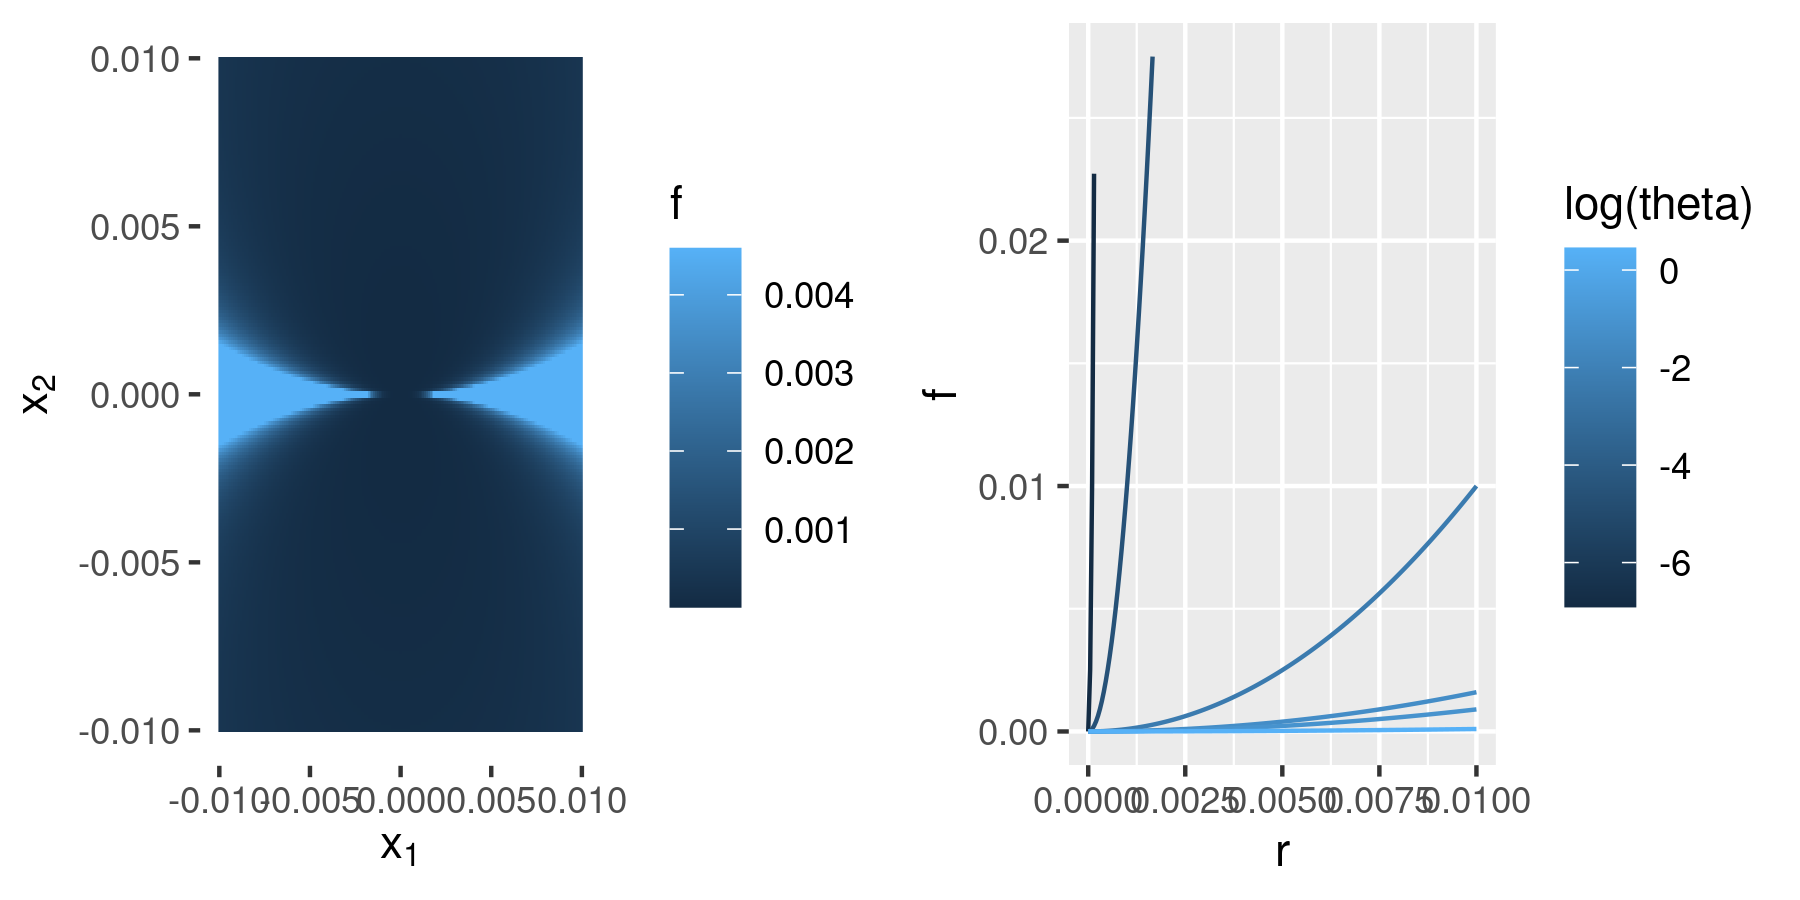
\includegraphics[width=0.980\linewidth,height=0.490\linewidth]{static_images/pathological_r2_example.png}
\caption{A plot of $f(x_1, x_2)$ from \exref{r2_pathological}.}
\figlabel{r2_pathological}
\centering
\end{figure}
%%%%%%%%%%%%%%%%%%%%%%%%%%%%%%%%%%%%%%%%%%%%%%%%%%%%%%%%%%%%%%%%%%%%%%%%%
%
\Figref{r2_pathological} contains a plot of $f(r, \theta)$, both over
$\mathbb{R}^2$ and along paths for particular choices of $\theta$.

We now show that $f$ has a directional derivative in every direction, but is not
Fr{\'e}chet differentiable.  By ordinary calculus, for any $\theta$,
$\fracat{\partial f(r, \theta)}{\partial r}{r=0} = 0$, so the directional
derivatives all exist and are identically $0$.  However, for any $r$, there
exists a $\theta(r)$ such that $r / |\sin(\theta(r))| = 1$.  For such a choice
of $\theta(r)$, the error in the linear approximation is $f(r, \theta(r)) - 0 =
1/2$, which does not go to zero as $r \rightarrow 0$.

\end{ex}
%%%%%%%%%%%%%%%%%%%%%%%%%%%%%%%%%%%%%%%%%%%%%%%%%%%%%%%%%%%%%%%%%%%%%%%%%

Fr{\'e}chet differentiability is only concerned with an infinitesimal
neighborhood.  The function can behave arbitrarily badly in a region just
outside the point at which the derivative is computed and retain Fr{\'e}che
differentiability. In this sense, Fr{\'e}chet differentiability is a desirable
but not sufficient requirement if we are interested in extrapolating using
linear approximations.  We illustrate this point in the

%%%%%%%%%%%%%%%%%%%%%%%%%%%%%%%%%%%%%%%%%%%%%%%%%%%%%%%%%%%%%%%%%%%%%%%%%
%%%%%%%%%%%%%%%%%%%%%%%%%%%%%%%%%%%%%%%%%%%%%%%%%%%%%%%%%%%%%%%%%%%%%%%%%
\begin{ex}\exlabel{r2_pathological_v2}
%
In \exref{r2_pathological} second derivative in a particular direction is given
by $\fracat{\partial^2 f(r, \theta)}{\partial r^2}{r=0} = \frac{1}{2 |\sin
\theta|}$, which can be made arbitrarily large by taking $\theta$ close to $0$
or to $\pi$.  We could modify $f(r, \theta)$ to be Fr{\'e}chet differentiable by
smoothly ``capping'' $1 / |\sin \theta|$ at some arbitrarily large value.
However, the ability to meaningfully extrapolate $f(r, \theta)$ in the direction
of a very large but finite second derivative will still be extremely limited.

In the context of \exref{r2_pathological}, fix some $0 < M < \infty$,
and define
%
\begin{align*}
%
\tilde{f}(r, \theta) := \begin{cases}
    f(r, \theta) & \textrm{when }\frac{1}{\abs{\sin(\theta)}} \le M \\
    0. & \textrm{when }\frac{1}{\abs{\sin(\theta)}} > M.
%
\end{cases}
%
\end{align*}
%
Then $\tilde{f}$ is continuous and Fr{\'e}chet differentiable at $r=0$. In this
case, for any $r$, $\sup_{\theta} r / |\sin(\theta(r))| = r / M$, so  both
$\lim_{r \rightarrow 0} \tilde{f}(r, \theta) \le \lim_{r \rightarrow 0} r^2 /
M^2 = 0$ and $\lim_{r \rightarrow 0} \tilde{f}(r, \theta) / r \le \lim_{r
\rightarrow 0}  r / M^2 = 0$.  (Note that $\tilde{f}$ is continuous only
at $r=0$, not on a ball centered at $0$.)

Despite being Fr{\'e}chet differentiable, the linear approximation may not
extrapolate well to any finite $r$.  In the direction $\theta = \sin^{-1}(1 /
M)$, the error of the linear extrapolation to any $r_0$ is still $\tilde{f}(r,
\theta) - 0 = M r_0^2$. Since Fr{\'e}chet differentiability requires only $M <
\infty$, the extraplation error can be arbitrarily large, even for Fr{\'e}chet
differentiable functions.

\end{ex}
%%%%%%%%%%%%%%%%%%%%%%%%%%%%%%%%%%%%%%%%%%%%%%%%%%%%%%%%%%%%%%%%%%%%%%%%%


\Exref{r2_pathological} is neither Fr{\'e}chet differentiable nor continuous,
whereas \exref{r2_pathological} is both Fr{\'e}chet differentiable and
continuous.  In general, however, Fr{\'e}chet differentiability is stronger than
continuity, in the sense that Fr{\'e}chet differentiability implies continuity,
but continuity does not imply Fr{\'e}chet differentiability \citep[Proposition
4.8 (d)]{zeidler:2013:functional}.  See also \citet[Example
1.9]{averbukh:1967:theory} for a simple example of a function on $\mathbb{R}^2$
that is continuous and directionally differentiable but not Fr{\'e}chet
differentiable.

The sort of pathology exhibited by \exref{r2_pathological, r2_pathological_v2}
requires some care to construct in $\mathbb{R}^2$, but requires some care to
avoid in infinite-dimensional spaces.  We now give an illustrative example in
the $\lp{p}$ spaces; since the result will be important for VB prior
sensitivity, we will state is as a lemma rather than merely an example.


%%%%%%%%%%%%%%%%%%%%%%%%%%%%%%%%%%%%%%%%%%%%%%%%%%%%%%%%%%%%%%%%%%%%%%%%%
%%%%%%%%%%%%%%%%%%%%%%%%%%%%%%%%%%%%%%%%%%%%%%%%%%%%%%%%%%%%%%%%%%%%%%%%%
\begin{ex}\exlabel{e_log_disocontinuous_v1}
%
Let $\q(\theta)$ and $\p(\theta)$ be densities relative to a continuous measure
$\lambda$.  Let $\gamma \in \lp{\p,p}$ with $1 \le p < \infty$, and define
%
\begin{align*}
%
f(\gamma) = \begin{cases}
\expect{\q(\theta)}{\log\left(1 + \gamma\right)}
    & \textrm{when }\inf_\theta \gamma(\theta) > -1 \\
-\infty & \textrm{otherwise}.
\end{cases}
%
\end{align*}
%
Then $f(\gamma)$ is trivially discontinuous at $\phiz$ since, for any $\gamma$
such that $\inf_\theta \gamma(\theta) = -\infty$,
%
\begin{align*}
%
f(\t \gamma) = -\infty \mathtxt{for any }\t > 0 \mathtxt{but} f(\phiz) = 0.
%
\end{align*}
%
\end{ex}
%%%%%%%%%%%%%%%%%%%%%%%%%%%%%%%%%%%%%%%%%%%%%%%%%%%%%%%%%%%%%%%%%%%%%%%%%

The problem with \exref{e_log_disocontinuous_v1} is not merely with
functions unbounded below, however.

%%%%%%%%%%%%%%%%%%%%%%%%%%%%%%%%%%%%%%%%%%%%%%%%%%%%%%%%%%%%%%%%%%%%%%%%%
%%%%%%%%%%%%%%%%%%%%%%%%%%%%%%%%%%%%%%%%%%%%%%%%%%%%%%%%%%%%%%%%%%%%%%%%%
\begin{ex}\exlabel{e_log_disocontinuous_v2}
%
In the setting of \exref{e_log_disocontinuous_v1}, assume further that, for any
$\epsilon \ge 0$, there exists a set $S_\epsilon$ such that $\p(S_\epsilon) \le
\epsilon$ and $\q(S_\epsilon) \ge \epsilon$.  Define
%
\begin{align*}
%
\tilde{f}(\gamma) = \begin{cases}
    f(\gamma) & \textrm{when }\inf_\theta \gamma(\theta) > -\infty \\
    0 & \textrm{otherwise}.
\end{cases}
%
\end{align*}
%
Now, with $\gamma$ such that $\inf_\theta \gamma(\theta) = -\infty$,
%
\begin{align*}
%
\tilde{f}(\t \gamma) = 0 \mathtxt{for any }\t > 0 \mathtxt{and} f(\phiz) = 0.
%
\end{align*}

However, $\tilde{f}$ is still discontinuous.  For any $\epsilon > 0$, let
$S_\epsilon$ be a set given in the assumption, and for $\delta > 0$, define
%
\begin{align*}
%
\gamma(\theta, \epsilon, \delta) :=
\begin{cases}
    %
    \delta - 1      & \textrm{ for }\theta\in S_\epsilon \\
    0      & \textrm{ for }\theta\notin S_\epsilon.
    %
\end{cases}
%
\end{align*}
%
Then $\gamma(\theta; \epsilon, \delta) \in \lp{\p,p}$ with.  Furthermore,
%
\begin{align*}
%
\norm{\gamma(\cdot;
\epsilon, \delta)}_{\p,p} =
    \left( \int_0^1 \phi(\theta)^p \p(\theta
)\lambda(d\theta)\right)^{1/p} \le{}& \epsilon^{1/p} (\delta - 1)  \mathand\\
%
\abs{\tilde{f}(\gamma(\cdot; \epsilon, \delta)) - \tilde{f}(\phiz)} =
    \expect{\q(\theta)}{\ind{\theta \in S_\epsilon}} \abs{\log(\delta)} \ge{}&
    \epsilon \abs{\log(\delta)}.
%
\end{align*}
%,
Take $\delta(\epsilon) = \exp(-\epsilon)$.  Then, for any sequence $\epsilon_n
\rightarrow 0$,
%
\begin{align*}
%
\abs{\tilde{f}(\phi(\cdot; \epsilon_n, \delta(\epsilon_n))) -
     \tilde{f}(\phiz)} \ge{} 1
\mathtxt{and}
\norm{\gamma(\cdot; \epsilon_n, \delta(\epsilon_n))}_p \rightarrow{} 0.
%
\end{align*}
%
So $\tilde{f}$ is discontinuous on an $\norm{\cdot}_p$ ball containing $\phiz$,
and cannot be Fr{\'e}chet differentiable.
%
\end{ex}
%%%%%%%%%%%%%%%%%%%%%%%%%%%%%%%%%%%%%%%%%%%%%%%%%%%%%%%%%%%%%%%%%%%%%%%%%

